\subsection{The LTCC Windows}

The LTCC windows that cover the upstream and downstream open frame of the box are a composite of
Tedlar/Mylar/Tedlar, see \F{windowDesign}. The Tedlar
material provides light tightness, while the Mylar adds the material strength necessary to withstand the gas pressure.

\begin{figure}
	\centering
	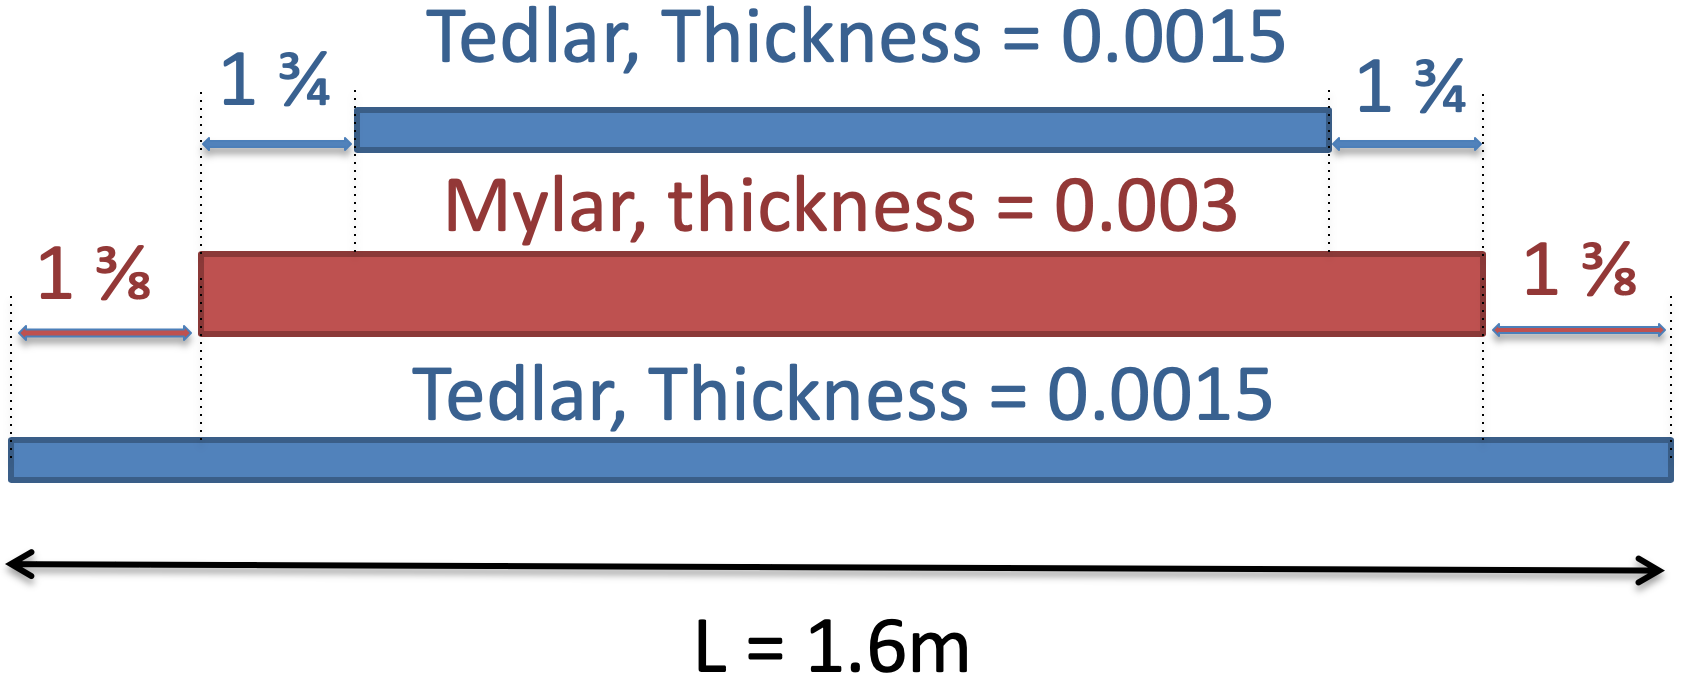
\includegraphics[width=1.0\columnwidth, keepaspectratio]{img/windowDesign.png}
	
\includegraphics[width=1.0\columnwidth, keepaspectratio]{img/blank.png}
	
\includegraphics[width=1.0\columnwidth, keepaspectratio]{img/windowSeaming.png}
	\caption{Top: the design of the LTCC Tedlar/Mylar/Tedlar window sandwich. The pyramid design allowed for the seaming shown at the bottom.
			 Bottom: the seaming design involves gluing Mylar to Mylar to ensure that the window stress is transmitted entirely to the Mylar. }
	\label{fig:windowDesign}
\end{figure}

The window was fabricated in two steps:

\begin{enumerate}
	\item lamination of Tedlar/Mylar/Tedlar rolls 1.6~m  wide
	\item seaming of the laminated strips into a square 4.8~m $\times$ 4.8~m window
\end{enumerate}

The lamination of the composite material, with dimensions outlined in \F{windowDesign} (top) was performed
at Madico \cite{madico}, where a sheet 400~m long was produced.

At Jefferson Lab rectangles were cut out of the laminated sheet, each 1.6~m wide and 4.8~m long.
To form a final 4.8~m $\times$ 4.8~m single LTCC window, three of the rectangles were seamed together
using G/Flex 655. The seam was load tested to withstand a pressure 10 times higher than that expected from
the gas flow and gas weight.

%\begin{figure}
%	\centering
%	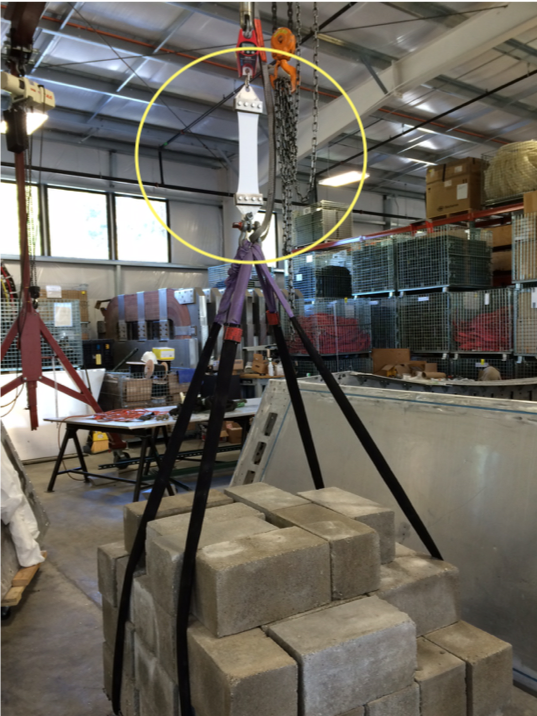
\includegraphics[width=1.0\columnwidth, height=1.0\columnwidth]{img/windowTest.png}
%	\caption{A window sample (white piece in the photograph) was tested with up to 388~lbs of load.
%          No significant damage was observed until rupture, which occurred at a load of 388~lbs, corresponding
%          to about 15,000~psi of stress on the window, about a factor of 10 higher than the stress during normal
%          operations of the detector.}
%	\label{fig:windowTest}
%\end{figure}

\subsubsection{Window Installation and Gas Leak Tests}

The installation of the window onto the box was achieved through gluing the window on the box sides using
G/Flex 655. The width of the window
attached with glue was 12~cm, to provide sufficient gluing area.
A photograph of the downstream window after installation is shown in \F{downstreamWindow}.

\begin{figure}
	\centering
	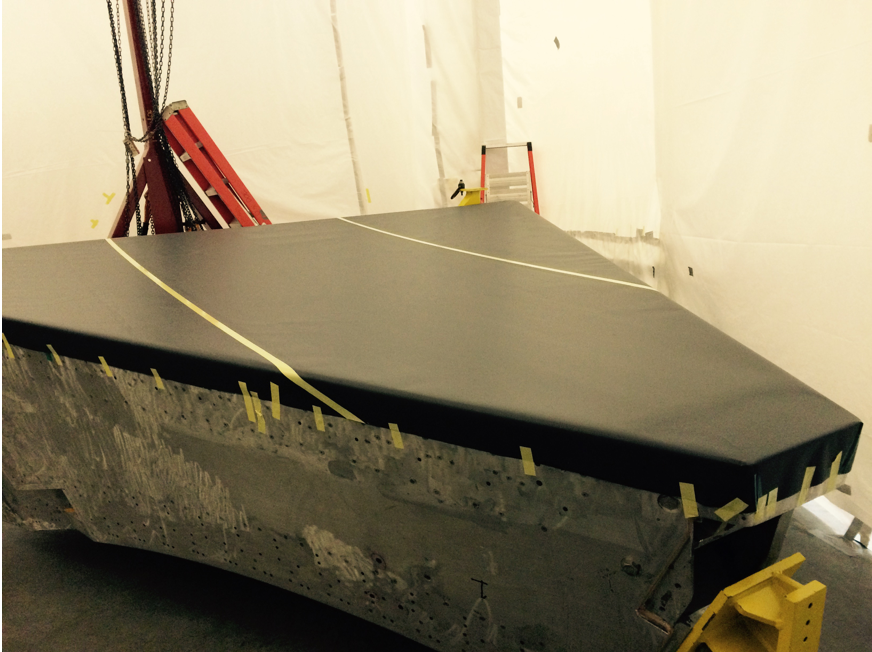
\includegraphics[width=1.0\columnwidth,keepaspectratio]{img/downstreamWindow.png}
	\caption{The downstream window of one LTCC sector during curing of the glue. The yellow strips protect the
          window seaming.}
	\label{fig:downstreamWindow}
\end{figure}

After curing of both the upstream and downstream windows, the LTCC box was filled with nitrogen gas to a pressure of
2~in of water.
Freon gas was pumped into the box and leaks were detected using a refrigerant leak detector. After the leaks were
sealed, the box was pressurized
for a 48 hour period to test the overall box gas tightness. This procedure was repeated after every movement of the LTCC boxes, as small
shifts of the frame walls had the potential to introduce additional leaks.

